\documentclass[
  bibliography=totoc,     % Literatur im Inhaltsverzeichnis
  captions=tableheading,  % Tabellenüberschriften
  titlepage=firstiscover, % Titelseite ist Deckblatt
]{scrartcl}

% Paket float verbessern
\usepackage{scrhack}

% Warnung, falls nochmal kompiliert werden muss
\usepackage[aux]{rerunfilecheck}

% unverzichtbare Mathe-Befehle
\usepackage{amsmath}
% viele Mathe-Symbole
\usepackage{amssymb}
% Erweiterungen für amsmath
\usepackage{mathtools}

% Fonteinstellungen
\usepackage{fontspec}
% Latin Modern Fonts werden automatisch geladen
% Alternativ zum Beispiel:
%\setromanfont{Libertinus Serif}
%\setsansfont{Libertinus Sans}
%\setmonofont{Libertinus Mono}

% Wenn man andere Schriftarten gesetzt hat,
% sollte man das Seiten-Layout neu berechnen lassen
\recalctypearea{}

% deutsche Spracheinstellungen
\usepackage[english]{babel}


\usepackage[
  math-style=ISO,    % ┐
  bold-style=ISO,    % │
  sans-style=italic, % │ ISO-Standard folgen
  nabla=upright,     % │
  partial=upright,   % │
  mathrm=sym,        % ┘
  warnings-off={           % ┐
    mathtools-colon,       % │ unnötige Warnungen ausschalten
    mathtools-overbracket, % │
  },                       % ┘
]{unicode-math}

% traditionelle Fonts für Mathematik
\setmathfont{Latin Modern Math}
% Alternativ zum Beispiel:
%\setmathfont{Libertinus Math}

\setmathfont{XITS Math}[range={scr, bfscr}]
\setmathfont{XITS Math}[range={cal, bfcal}, StylisticSet=1]

% Zahlen und Einheiten
\usepackage[
  locale=DE,                   % deutsche Einstellungen
  separate-uncertainty=true,   % immer Unsicherheit mit \pm
  per-mode=symbol-or-fraction, % / in inline math, fraction in display math
]{siunitx}

% chemische Formeln
\usepackage[
  version=4,
  math-greek=default, % ┐ mit unicode-math zusammenarbeiten
  text-greek=default, % ┘
]{mhchem}

% richtige Anführungszeichen
\usepackage[autostyle]{csquotes}

% schöne Brüche im Text
\usepackage{xfrac}

% Standardplatzierung für Floats einstellen
\usepackage{float}
\floatplacement{figure}{htbp}
\floatplacement{table}{htbp}

% Floats innerhalb einer Section halten
\usepackage[
  section, % Floats innerhalb der Section halten
  below,   % unterhalb der Section aber auf der selben Seite ist ok
]{placeins}

% Seite drehen für breite Tabellen: landscape Umgebung
\usepackage{pdflscape}

% Captions schöner machen.
\usepackage[
  labelfont=bf,        % Tabelle x: Abbildung y: ist jetzt fett
  font=small,          % Schrift etwas kleiner als Dokument
  width=0.9\textwidth, % maximale Breite einer Caption schmaler
]{caption}
% subfigure, subtable, subref
\usepackage{subcaption}

% Grafiken können eingebunden werden
\usepackage{graphicx}

% schöne Tabellen
\usepackage{tabularray}
\UseTblrLibrary{booktabs, siunitx}
\usepackage{longtable}

\DefTblrTemplate{contfoot-text}{normal}{Weiter auf der nächsten Seite}
\SetTblrTemplate{contfoot-text}{normal}
\DefTblrTemplate{conthead-text}{normal}{(Fortsetzung)}
\SetTblrTemplate{conthead-text}{normal}

% Verbesserungen am Schriftbild
\usepackage{microtype}

% Literaturverzeichnis
\usepackage[
  backend=biber,
]{biblatex}
% Quellendatenbank
\addbibresource{lit.bib}
\addbibresource{programme.bib}

% Hyperlinks im Dokument
\usepackage[
  german,
  unicode,        % Unicode in PDF-Attributen erlauben
  pdfusetitle,    % Titel, Autoren und Datum als PDF-Attribute
  pdfcreator={},  % ┐ PDF-Attribute säubern
  pdfproducer={}, % ┘
]{hyperref}
% erweiterte Bookmarks im PDF
\usepackage{bookmark}

% Trennung von Wörtern mit Strichen
\usepackage[shortcuts]{extdash}

% Schriftfarbe ändern
\usepackage{xcolor}

\begin{document}

\section*{\Huge \textbf{Checkerboard Submission}}

\subsection*{Problem 1}

The smallest amount of layers and neurons in order to give a good fit result consists of only one layer and three neurons as seen in \autoref{fig:Fig01}.

\begin{figure}[H]
  \centering
  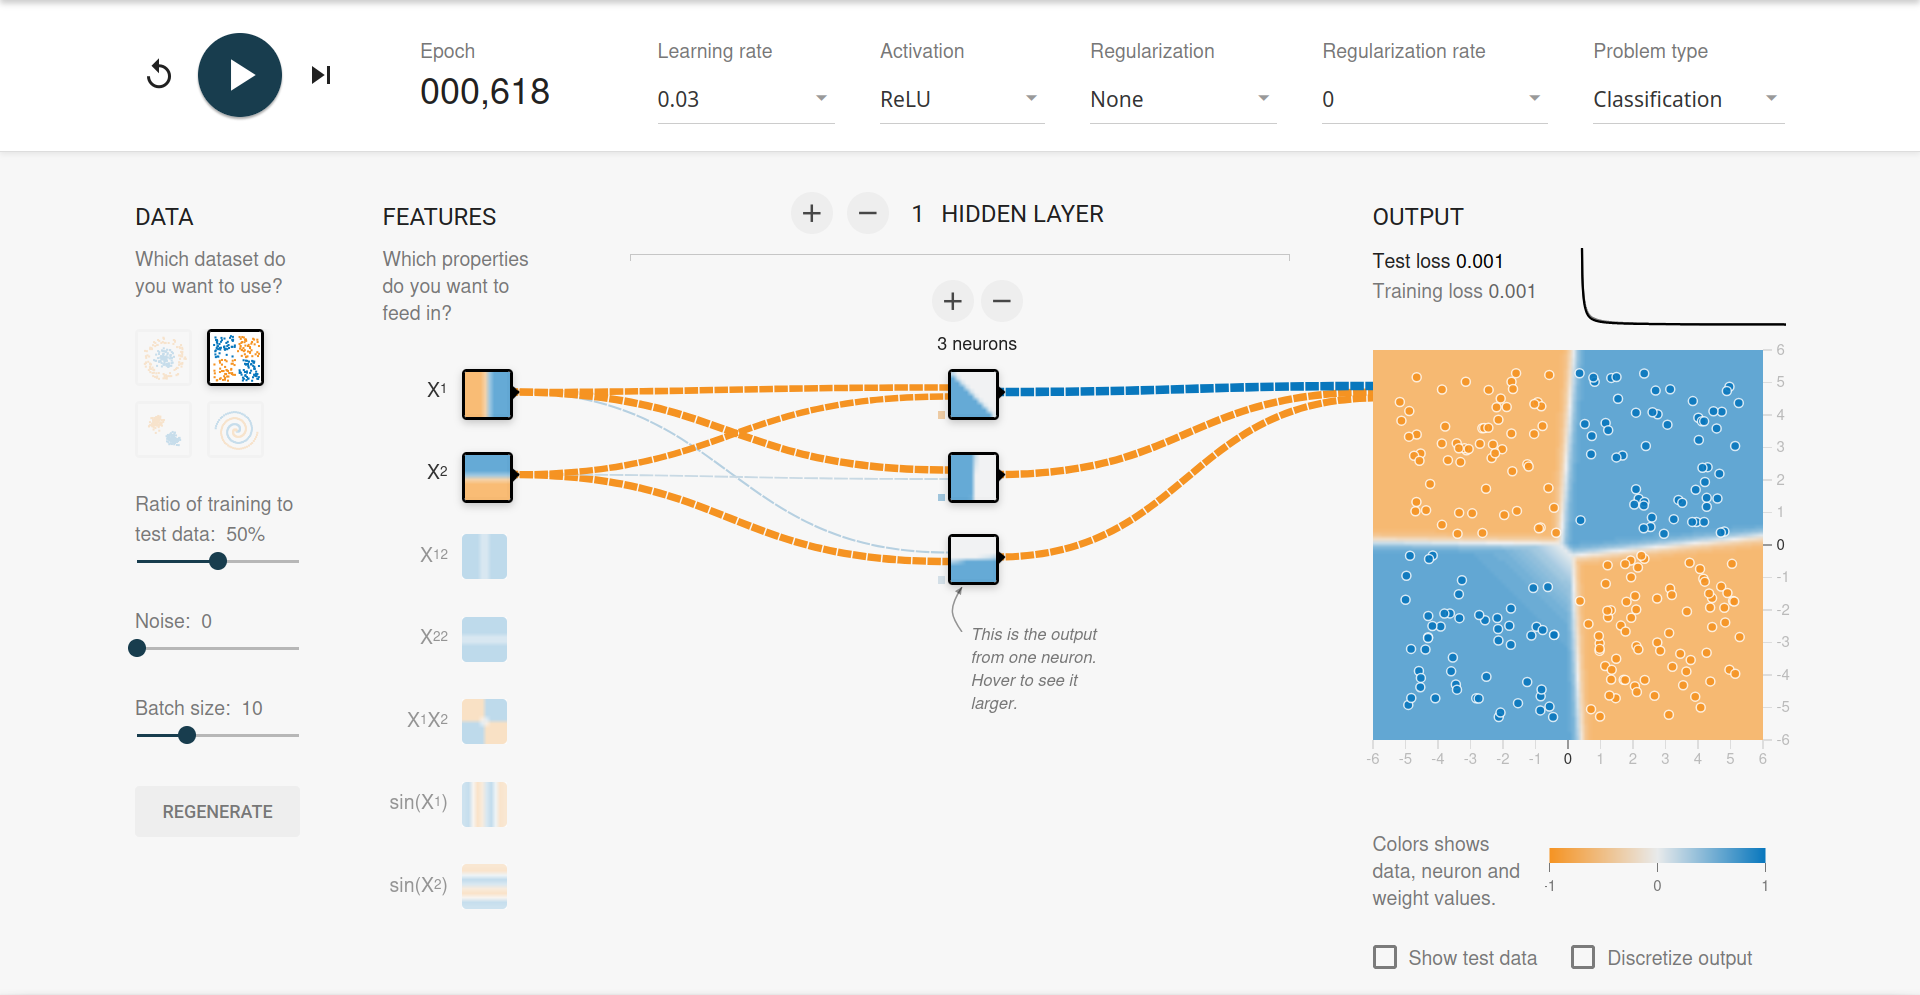
\includegraphics[width=\textwidth]{Screenshot_1.png}
  \caption{Neural Network consisting of one layer and three neurons to fit the checkerboard.}
  \label{fig:Fig01}
\end{figure}

Changing the amount of layers and neurons may increase the quality of the fit, which is already quite good with a loss of $\qty{0.001}{}$.
On the other side, it is also possible to make the fit worse. For example a neural network with two layers and two neurons each, as seen in \autoref{fig:Fig02}, is not able to
identify the scatter plot at all.

\begin{figure}[H]
  \centering
  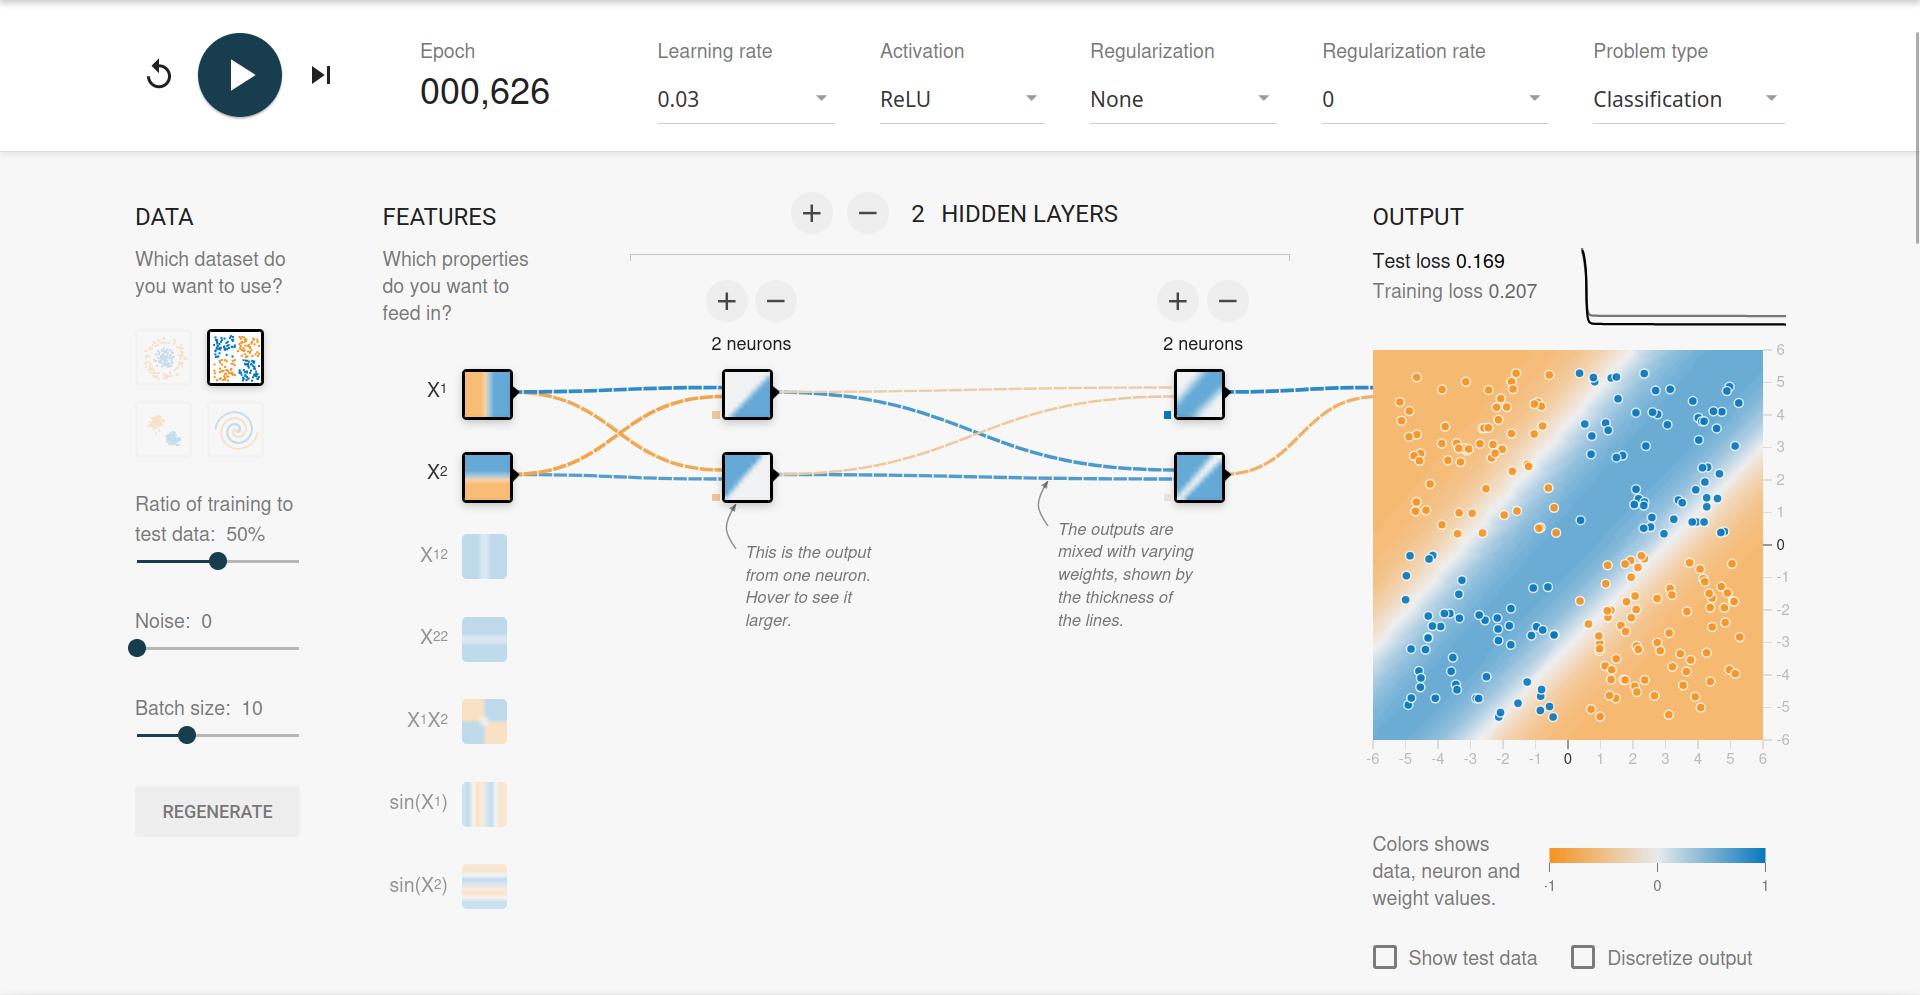
\includegraphics[width=\textwidth]{Screenshot_2.png}
  \caption{Neural Network consisting of two layers and two neurons each to fit the checkerboard.}
  \label{fig:Fig02}
\end{figure}

The loss function is way higher, and it is directly visible, that the checkerboard has not been identified at all. 
The shown fit in \autoref{fig:Fig02} is merely an example of this neural network set, since repeating the training with the same network structure and settings may vary the result as seen in the second problem.

\newpage
\subsection*{Problem 2}

When the neural network is trained with the same settings multiple times in a row, different results and fits may occur. Some of them can be seen in \autoref{fig:Fig03} as examples.

\begin{figure}[!htp]
  \begin{subfigure}[inner-pos=t]{0.5\textwidth}
      \centering
      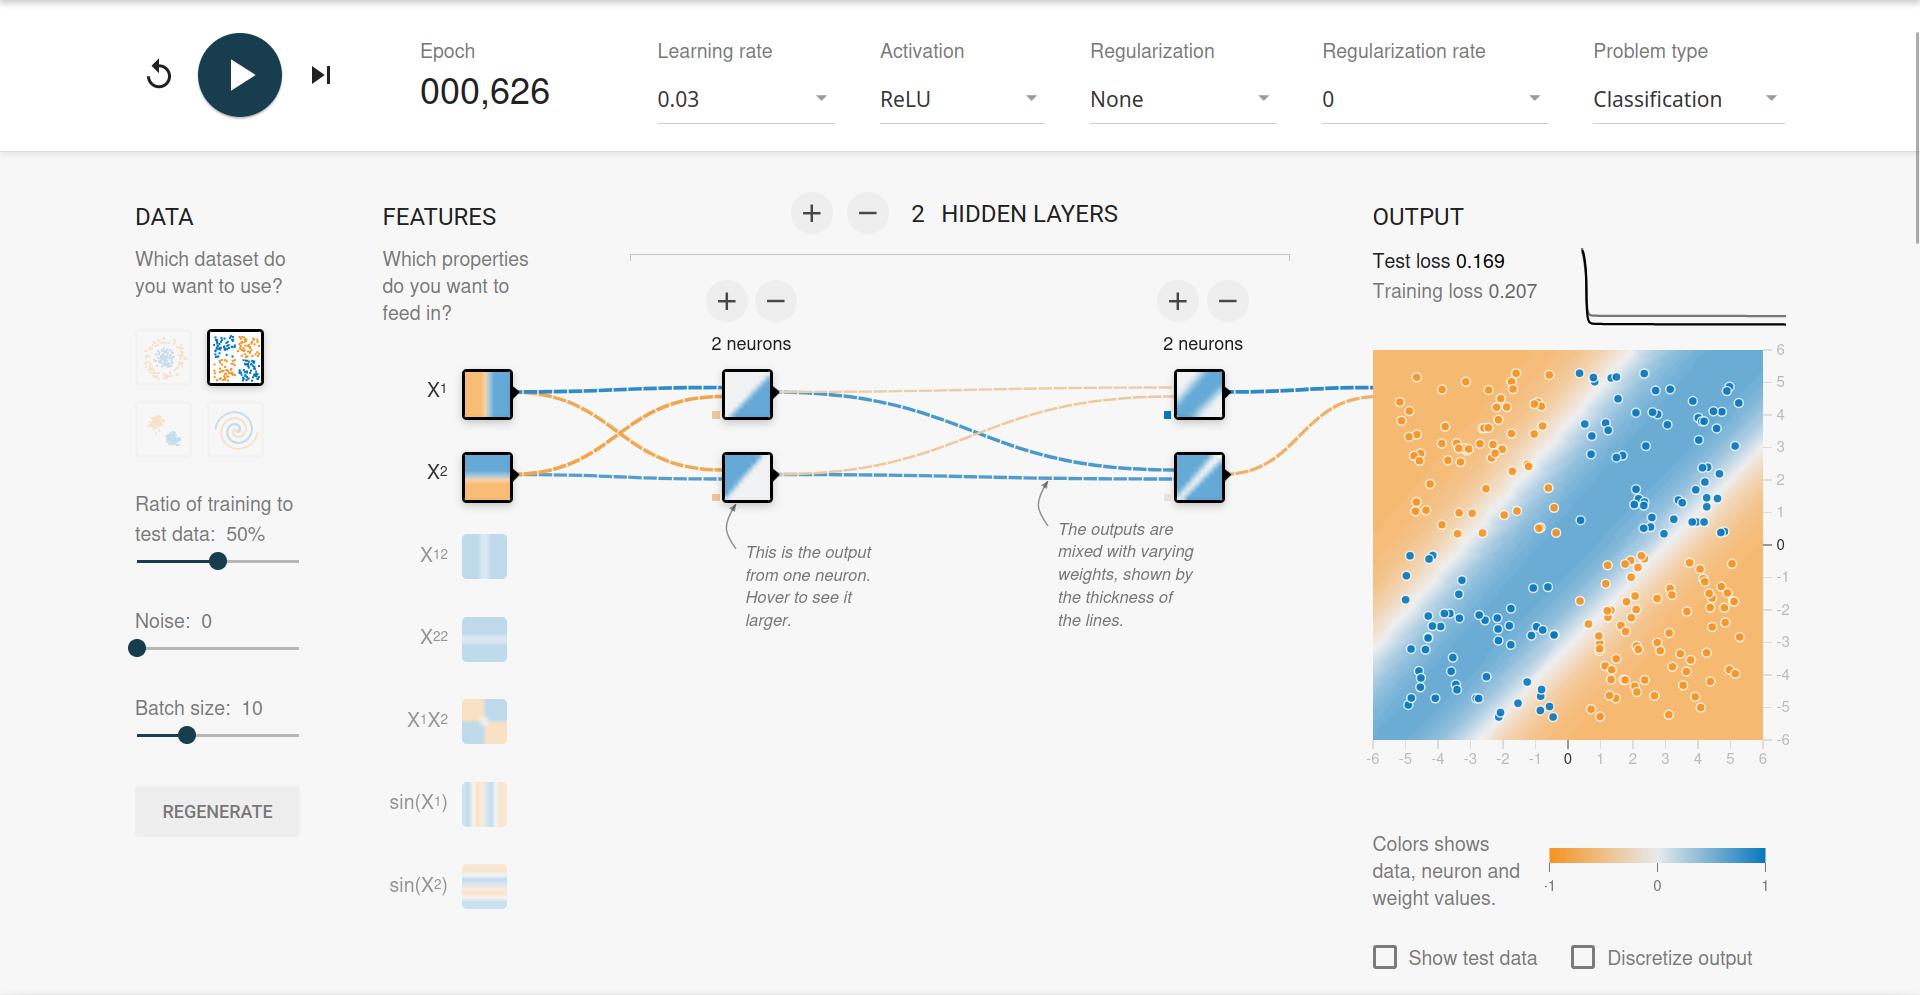
\includegraphics[width=0.98\textwidth]{Screenshot_2.png}
  \end{subfigure}
  \hfill
  \begin{subfigure}[inner-pos=t]{0.5\textwidth}
      \centering
      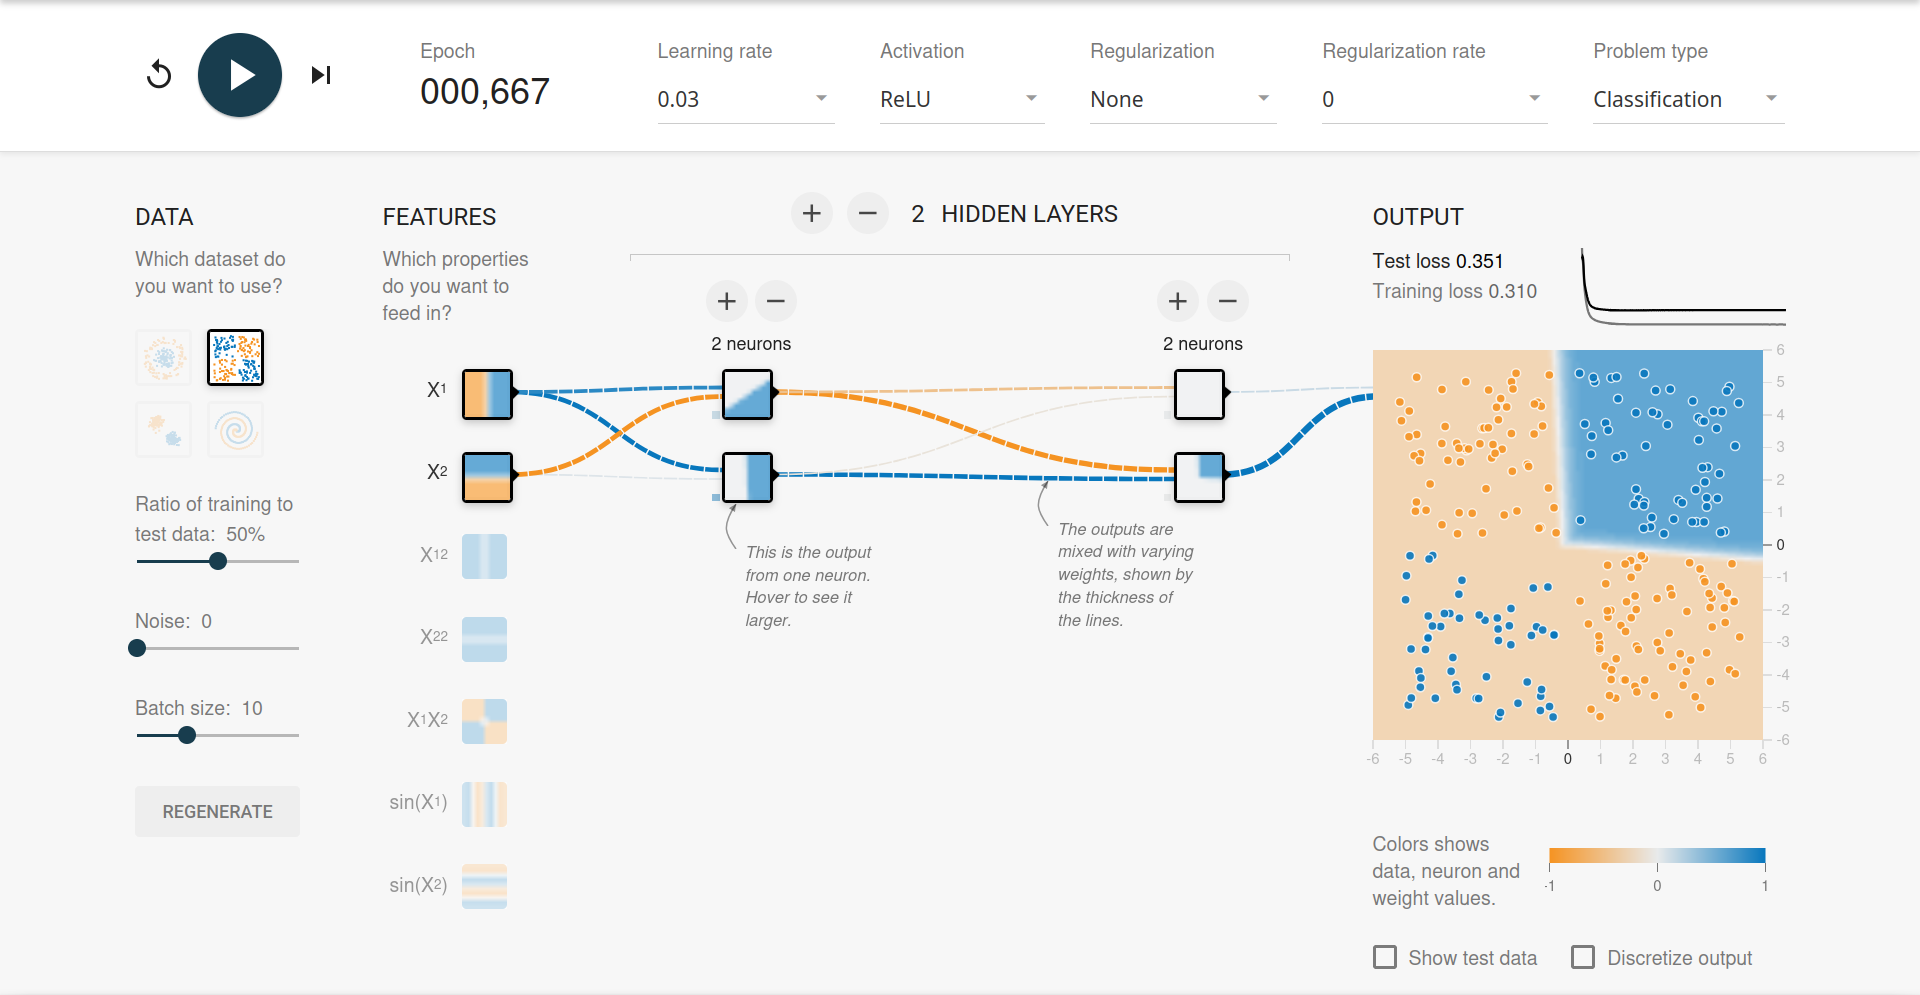
\includegraphics[width=0.98\textwidth]{Screenshot_3.png}
  \end{subfigure}
\end{figure}
\vskip -2em
\begin{figure}[!htp]\ContinuedFloat
  \begin{subfigure}[inner-pos=t]{0.5\textwidth}
      \centering
      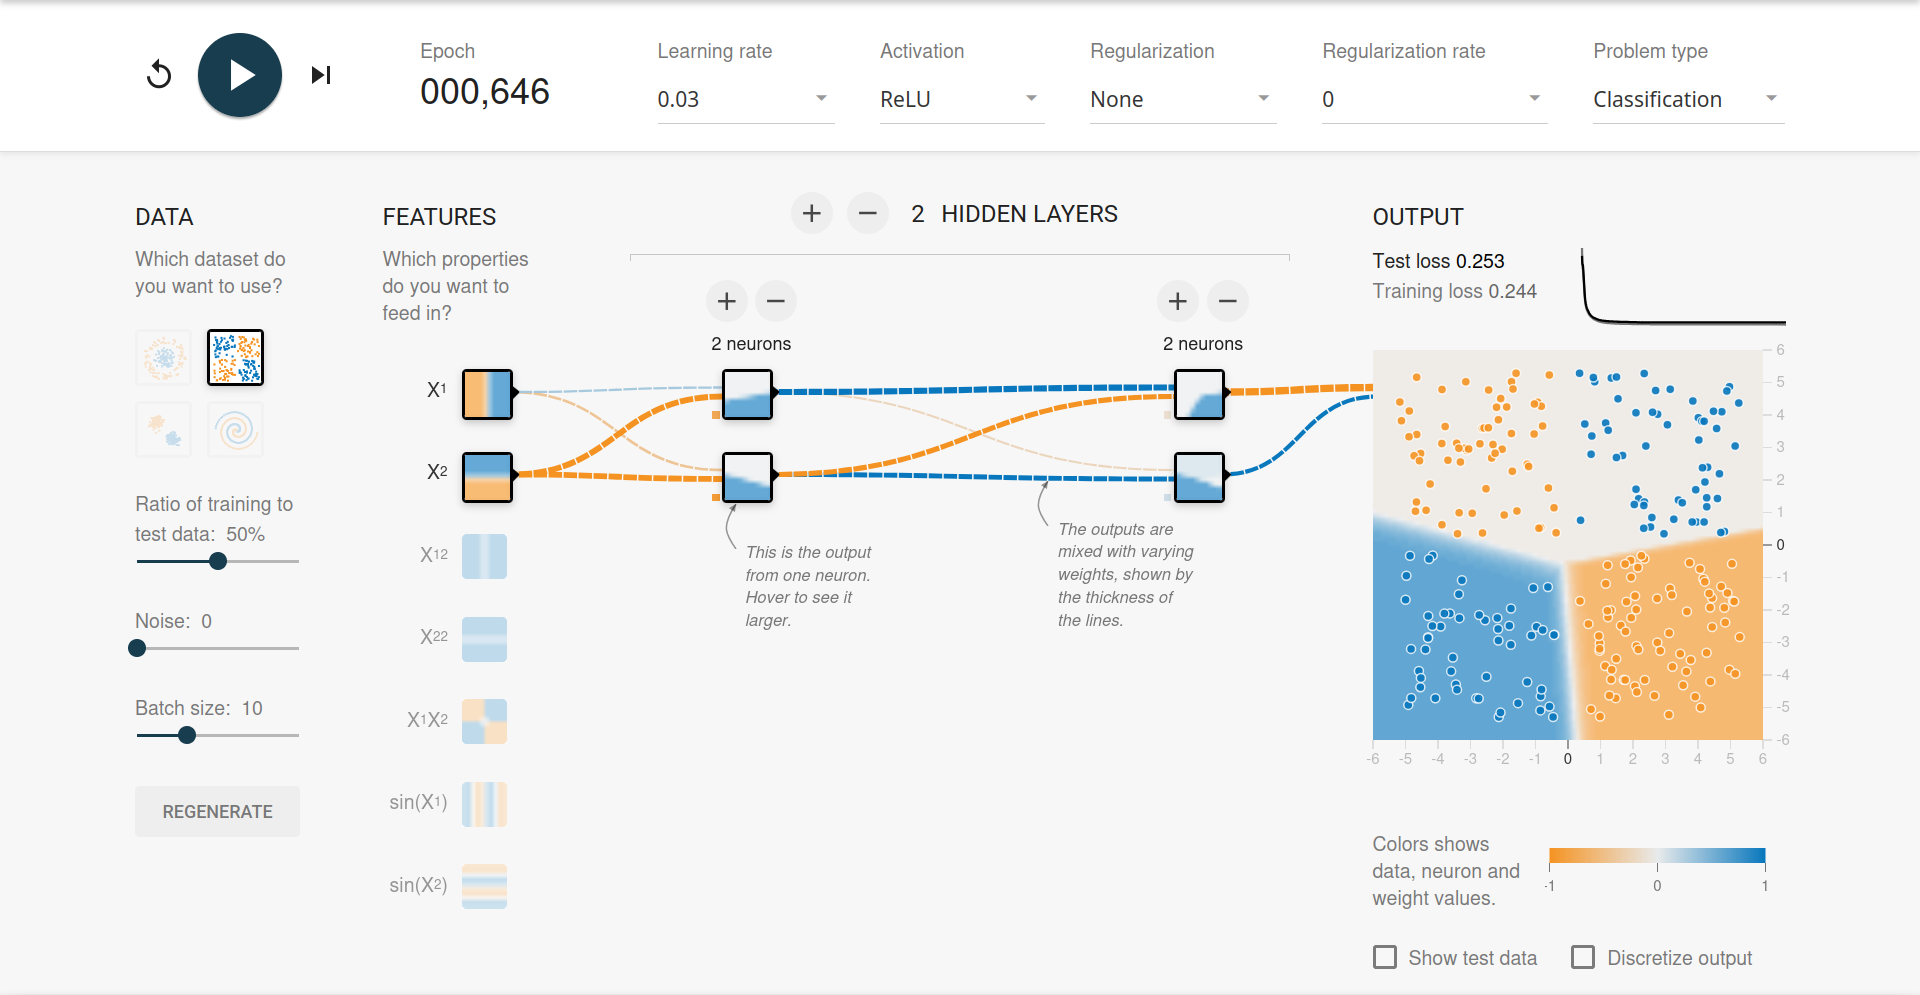
\includegraphics[width=0.98\textwidth]{Screenshot_4.png}
  \end{subfigure}
  \hfill
  \begin{subfigure}[inner-pos=t]{0.5\textwidth}
      \centering
      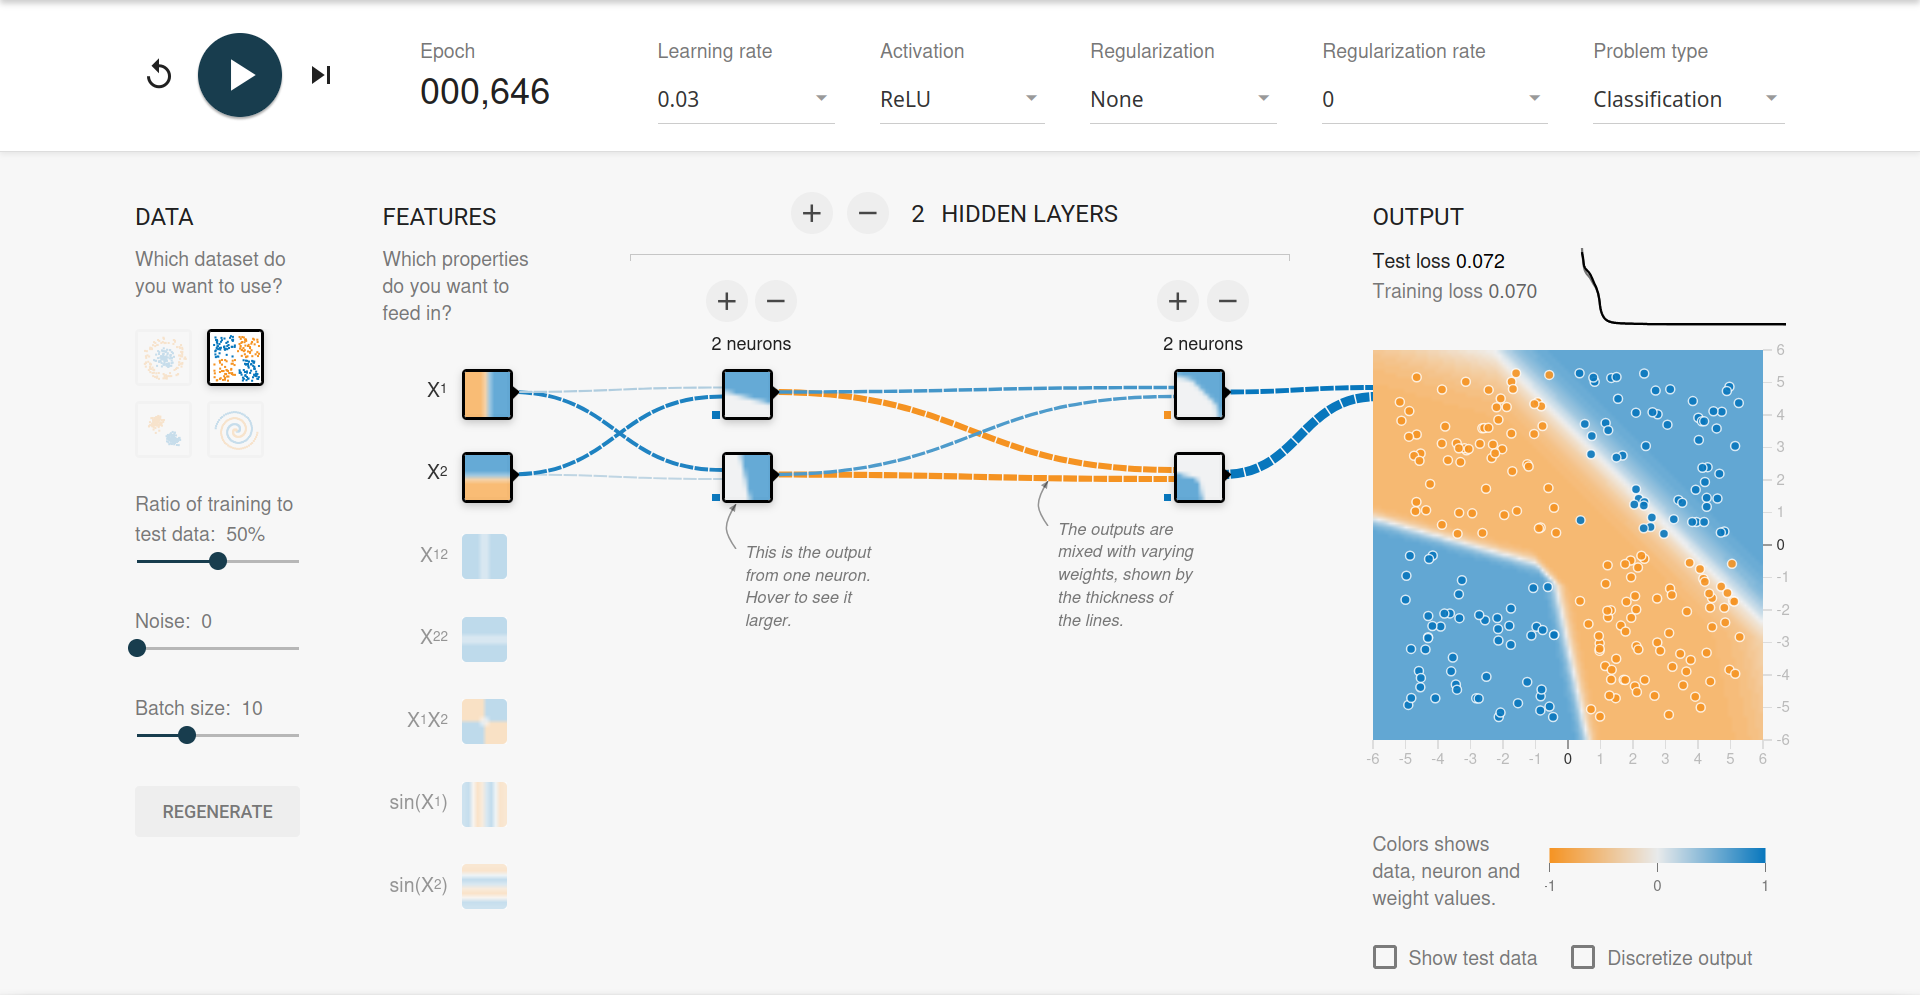
\includegraphics[width=0.98\textwidth]{Screenshot_5.png}
  \end{subfigure}
  \caption{Neural Network consisting of two layers and two neurons each to fit the checkerboard. The different fits result from different training iterations.}
  \label{fig:Fig03}
\end{figure}

This happens due to different weights that the algorithm applies to the different neurons. 
Even though the fit in \autoref{fig:Fig01} is obviously the best one to describe the checkerboard, the neural network also finds different local minima for the fit, which result in the different decision boundaries in \autoref{fig:Fig03}.

\newpage
\subsection*{Problem 3}

Changing the different input features strongly changes the quality of the fit. 
While the $\sin(X^1)$ and $\sin(X^2)$ make the fit worse in a way, that it tries to introduce fits following a waveform to the decision boundaries.
On the other side, adding the $X^1X^2$ feature to the neural network, strongly increases its quality. Even a network consisting of no hidden leyer can now fit the checkerboard quite well as seen in \autoref{fig:Fig04}.

\begin{figure}[H]
  \centering
  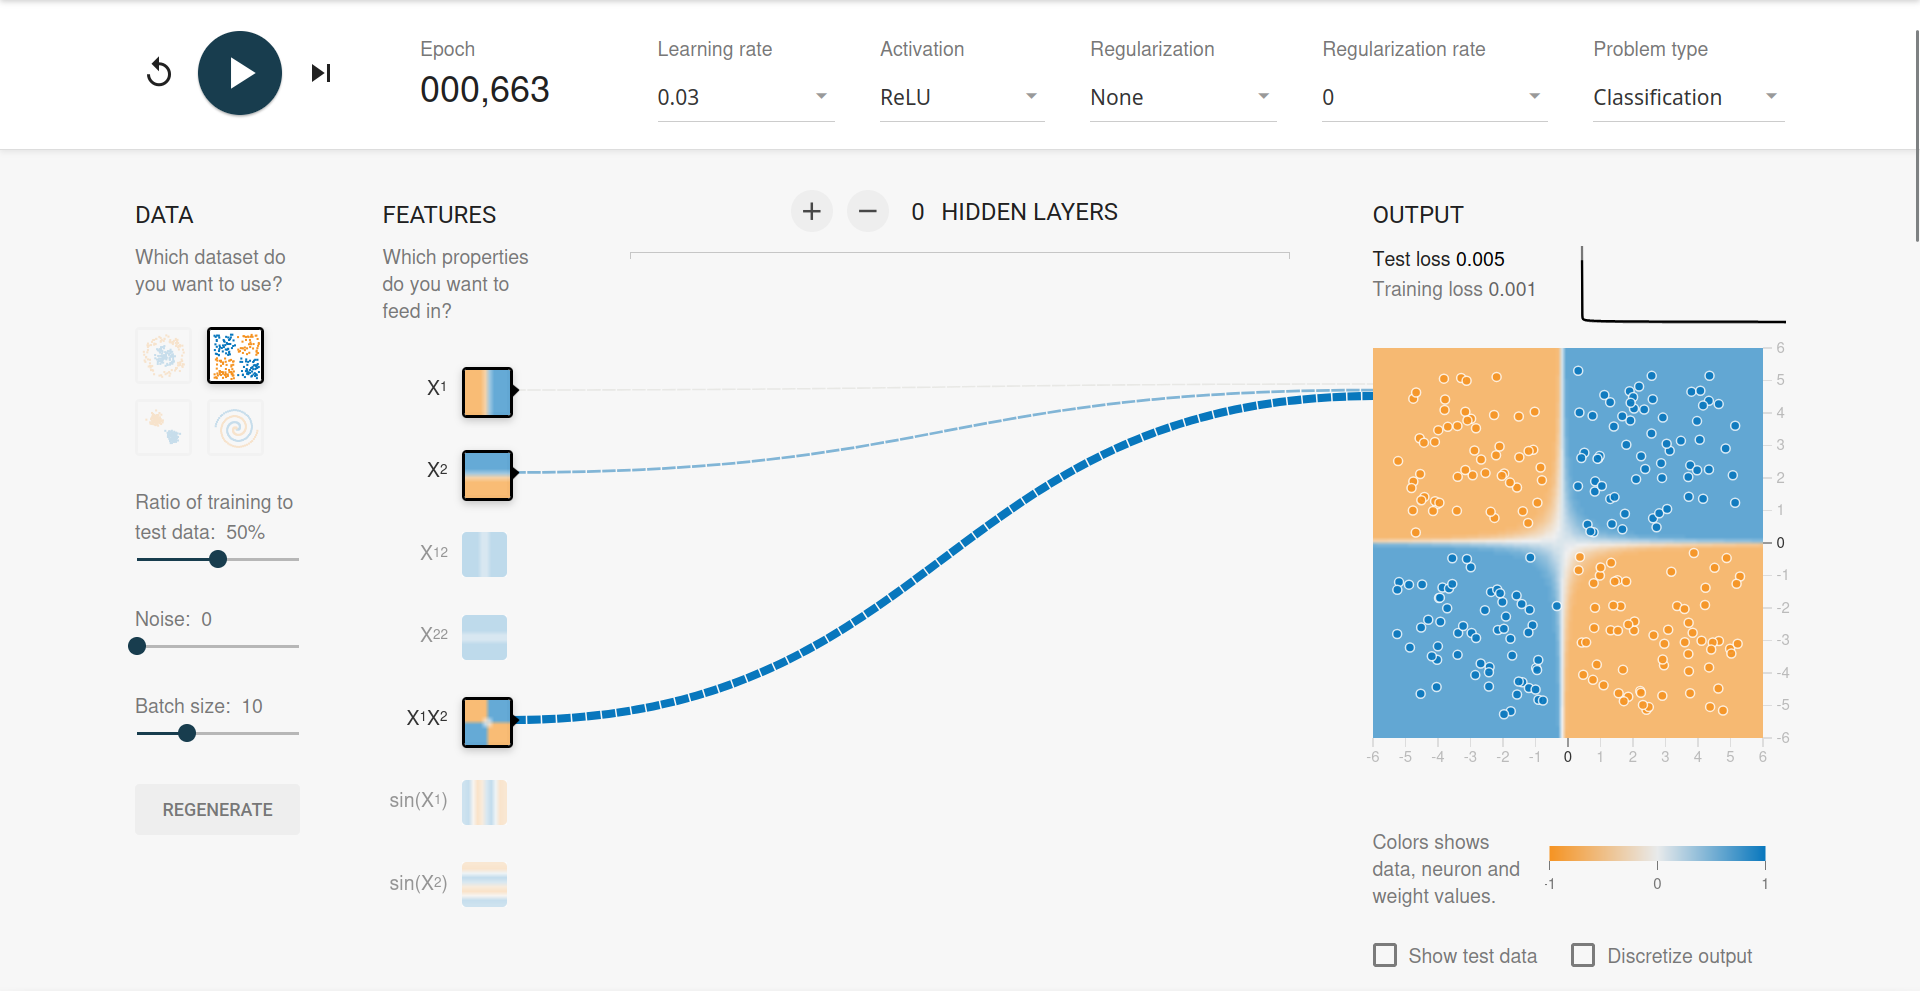
\includegraphics[width=\textwidth]{Screenshot_6.png}
  \caption{Neural Network without any hidden layer to fit the checkerboard.}
  \label{fig:Fig04}
\end{figure}

But since the $X^1X^2$ feature looks identical to the checkerboard, an improvement of the network with it was expectable.

\end{document}
